%%% -*-LaTeX-*-

\chapter{The Multi-cluster Trading Mechanism}

As the adoption of multi-cluster environments accelerates and the
infrastructure continues to evolve to support more use cases, there is an
opportunity to develop tools that leverage existing networking solutions to
optimize inter-cluster interactions in a multi-cluster environment. . Given the
broad definition of a multi-cluster environment, we define our specific context
as one in which clusters are discoverable to one another and implement the
trading mechanism's API.

We argue that it is possible to increase cluster resource utilization, decrease
average job completion time, and reduce cost by providing clusters with a
resource trading mechanism that allows the virtual sharing of resources across
clusters. 

In this chapter we present the system design, discuss the role of the scheduler
in the mechanism, explain what user-defined policies and rules are, and
describe the design of the trader itself. The following figure illustrates the
mechanism's design and will be elaborated upon in the subsequent sections: 

\begin{figure}[H]
  \centerline{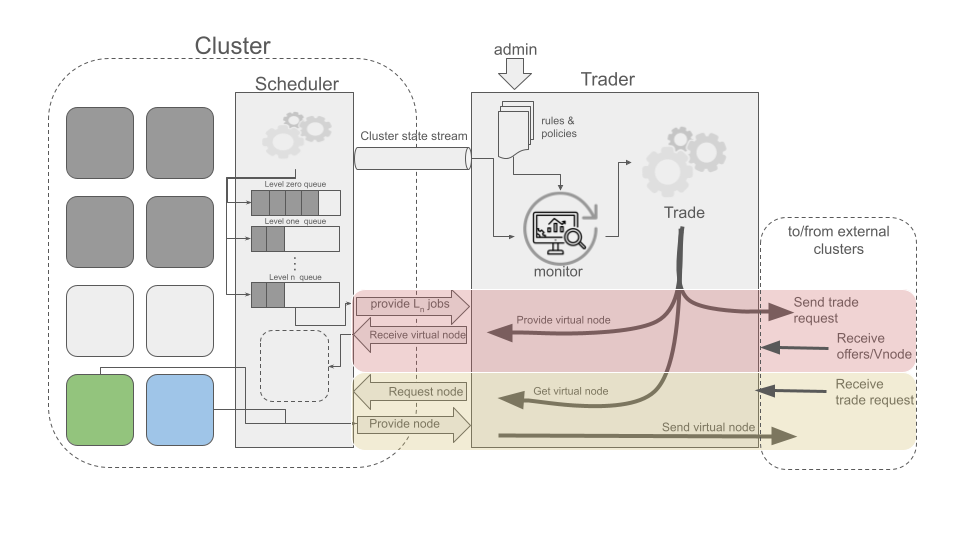
\includegraphics[scale=0.45]{figures/system-diagram}}
  \caption{System architecture showing the various compononents of the trader,
    and how it connects to a cluster. Red section represents the procedure
    requesting resources and the yellow section depicts the procedure of
    providing resources to external clusters. squares represents the node in
    the host cluster. Dark gray nodes represent localy utilized nodes and light
    gray nodes represent free local nodes. Green and blue nodes represent
    resources    provided to external clusters and the dotted square is a
    virtual node received from an external cluster} 
  \figlabel{fig1}
\end{figure}

\section{Scheduler}
% introducing the notion of minimal intursivity
\subsection{Requirements}

Cluster scheduling have been widely studied and remains a prominent area of
research \cite{hindman_mesos_nodate, zaharia_delay_2010, patel_what_2022,
li_lyra_2023, qiao_pollux_nodate, schwarzkopf_omega_2013,
karanasos_mercury_2015, delgado_hawk_2015}. Our objective concerning scheduling
is not to replace the clusters' scheduling algorithm nor interfere with its
scheduling decisions, but to improve cluster performance while minimizing
friction the mechanism's components. This minimally intrusive approach allows
us to maintain the scheduler's independence from the mechanism and confine all
of the mechanism's logic and interactions to its components.

The scheduler's role in the mechanism comprises of transmitting cluster state
as well as supplying and receiving resources needed for trades. Cluster state are
measurements necessary for making informed trading decisions. These metrics are
typically collected in cluster schedulers for performance analysis and
monitoring and include wait time, infrastructure cost, and utilization.

\noindent Providing and receiving resources are an extension of the cluster's
ability to add new nodes and allocate resources on existing ones. 

This lays the groundwork for the general requirements for a scheduler to
operate in the mechanism. With that being said, we now present our scheduling
algorithm and discuss the underlying design decisions. 

\subsection{Design}
% delay scheduling 

The foundation of our scheduling algorithm is delay scheduling
\cite{zaharia_delay_2010}; it establishes a clear spectrum of how far away jobs
can be scheduled from their data which we extend to encompass running jobs
outside of the cluster and on external cluster. In delay scheduling, a job is
first enqueued at the lowest level, queue zero, allowing it to only be
scheduled on the node where its data is located. As the scheduler fails to
schedule it in close proximity to its data, the job is subsequently bumped up
to higher queue levels, allowing the scheduler to schedule the job further away
from its data as the job wait time increases. Consequently the leveling
represents the job's expectated distance from its data. This notion of proximity
and gradual drifting is extended to include external clusters in our mechanism.
Jobs with high wait times already anticipating poor data locality would be the
ones more likely to be scheduled on an external cluster. This insures fair
scheduling even as we extend the scope of scheduling to a multi-cluster
environment. These jobs would also incur the least percentage reduction in
performance when scheduled on an external cluster compared to being run
locally.

\figref{fig1} illustrates the architecture of the scheduler described here. The
different queues represent different levels a job can be in. Colored squares
represent nodes running external jobs and the grey ones represent nodes running
local jobs. The incoming and outgoing arrows represents the exposed interface
the trader utilizes to communicate with the scheduler and will be further
explained in the next section.

%Of course, more analysis could go in deciding what jobs would better fit being
%exported to other clusters like jobs demanding less communiication with other
%jobs in the cluster, jobs with less data dependency, ..., but this is out of
%scope of this thesis.


% research idea: data locality-aware scheduling research is trying to get the
% jobs scheduled next to data, no study i encountered actually socres the
% sensitivity of the jobs in relation to other jobs in the cluster. (probably
% for fairness concerns) but might be an interesting project to work on. 

%This presents us with a clean heuristic when calculalting resources needed for
%trading. As the level of the of what to include in our 


\section{Trader} \label{trader}

The trader is the core component of the mechanism, facilitating the
exchange of resources between clusters and encapsulating all trading logic. 

This exchange is bidirectional, allowing a cluster to receive external
resources and allocate its own resources to other clusters. Clusters 
communicate solely through their traders, which are configured by the
cluster adminstrator. 

Traders can either operate in a cooperative or opportunistic manner. In a
cooperative trading environment, furthers the overall performance of
participating clusters. A straightforward use-case for this model is
organizations with multiple clusters; allowing the exchange of resources
benefits the organization as a whole. On the other hand, the opportunistic
model facilitates trading between self-serving clusters by introducing an
incentive in a trade. Traders evaluate the cost and profit of participating in
a trade and this cost-benefit analysis motivates resource sharing.

The trader is responsible for keeping the cluster's state in alignment with a
desired state. As shown in the figure, the trader establishes a cluster state
stream with the scheduler, continously receiving up-to-date cluster
information. This information includes the overall cluster utilization, average
job completion time, and current resource costs. This stream enables the trader
to monitor and make trading decisions based on the current state of the
cluster. The desired state is declared through a set of dynamically
configured rules passed to the trader.

\begin{figure}[H]
  \begin{lstlisting}[language=go]
    type Rule struct {
      Condition: // desired state to maintain
      Action: // algorithm to use
      Broken(cluster state, condition) bool
    } 
  \end{lstlisting}
  \caption{Rules}
\end{figure}

The rule's condition represents the desired state of a measurement sent by the
scheduler to the trader such as maintaining utilization below a certain
threshold. The rule implements a Broken method, enabling the trader trader to execute 
an action when the actual cluster state deviates from the desired state. As the
trader continously monitors the cluster state, it runs the broken methods of
all rules to determine whether any have been violated.

The following algorithm details what happens when a rule is broken, also marked
in red in \figref{fig1} 

\begin{figure}[H]
\begin{algorithm}[H]
\caption{Outgoing Trading Algorithm}
\begin{algorithmic}
  \Procedure{Trade}{$R_b$} \Comment{$R_b$ = broken rule}
    \State $R_{action} \gets Action(R_b)$
    \State $level_N Jobs \gets GetJobs(n)$ \Comment{get from scheduler}
    \State $virtualNodeSize \gets calculateNodeSize(R_{action}, level_N Jobs)$
    \If{Incentivized}
      \State $incentive \gets calculateIncentive()$
    \EndIf
    \For{traders in multi-cluster environment}
      \State $contract \gets SendTradeRequest(virtualNodeSize, incentive)$
    \EndFor
    \State $contracts \gets ReceiveTradeResponses$ \Comment{list of approved contracts}
    \State \textbf{return} $contract_{best}$\Comment{best virtual node is sent to scheduler}
  \EndProcedure
\end{algorithmic}
\end{algorithm}
\caption{Outgoing Trading Algorithm}
\end{figure}

A virtual node is an abstraction that encapsulates the resources requested from
an external cluster. It encompasses the needed resources, time, and any
additional constraints such as specific hardware or operating system
requirements for job execution. This abstraction represents the total resources
needed by the trader, and can be mapped onto multiple nodes within the external
cluster, collectively fulfilling the resource requirements of the virtual node.

% The trader specifies the smallest partition it accepts in the
% contract, usually the size of the smallest job it has in the jobs list.

When a rule is broken, the trader's initial task is to estimate the size of the
virtual node. The resource estimate is calculuated by first retreiving the last
level jobs from the scheduler, comprising of jobs with the highest wait times.
The rule's action variable specifies the algorithm to be used for the estimation.
Currently, there are two methods to estimate the resource request:

\begin{enumerate}

  \item \textbf{Incremental Job Packing:} This method employs a greedy approach
    to stack jobs efficiently over time on the requested virtual node. It
    starts with the oldest job in the $level_N$ queue and incrementally
    includes one job at a time to the estimation, adjusting the size of the
    virtual node to accomadate each new job. The goal is to minimize virtual
    node size while ensuring the highest number of jobs are accounted for
    before a constraint is reached.

  \item \textbf{Simultaneous Job Initiation:} This approach estimates the size
    of the node assuming all jobs will start simultaneouslt when the virtual
    node is becomes available. It incrementally includes each job at the start
    time of the virtual node, increasing its size until a constraint is
    reached. 

\end{enumerate}

Incremental job packing enables the trader to decrease the size of the virtual
node which in turn reduces the cost of the trade and improves the likelihood of
approval. However, this approach incurs higher computation cost and may result
in slower performance gain from the trade. In contrast, simultaneous job
initiation increases the potential benefit from a trade but comes at a higher
cost per node and lower computation cost.

Virtual node constraints define the limits on resource allocation, and include
parameters such as the maximum number of cores, amount of memory, and time to
be requested per node. In case of opportunistic environments the contraints
also include a budget, imposing a limit on the incentive send per node.

%version more appealing on a lower budget. It would be advantagous to request
%resources from another trader if it is cheaper than scaling up the cluster
%size. [Might want to introduce budgeting a bit earlier]

The incentive calculation is influenced by factors including the cost of
internally scaling up the cluster (if possible), the severity of the broken 
rules, and the allocated trading budget.

The trader then broadcasts a contract proposal to all participating clusters
and waits for their responses. Upon receiving the approved contracts, the
trader ranks them based on multiple criterion like cost, proximity, and prior
trade history. The trader then approves the most advantageous contract,
requests the access to the virtual node, and subsequently provide the necessary
information to the scheduler.

The trader is also responsible for accepting or rejecting incoming trade
requests. This functionality is outlined in the yellow section in \figref{fig1}
and detailed in the following algorithm: 

\begin{figure}[H]
\begin{algorithm}[H]
\caption{Incoming Trading Algorithm}
\begin{algorithmic}
  \Procedure{ApproveTrade}{$contract$} \Comment{$contract$ = trade request}
    
    \If{$ ccs \leq contract.resources$} \Comment{ccs = current cluster state}
      \State \textbf{return} $false$ \Comment{couldn't approve trade}
    \EndIf

    \For{$P$ in Policies}
      \If{$P(ccs, T_{request}) \not= true$} 
      \State \textbf{return} $false$ \Comment{couldn't approve trade}
      \EndIf
    \EndFor
    \State $contract_r \gets sendTradeResponse$ \Comment{$contract_r$ = trade response}
    \State $contract_a \gets receiveContractApproval$ \Comment{$contract_a$ = approved trade}

    \State $virtualNode \gets getVirtualNode(T_{request})$ \Comment{from scheduler}    
    \State \textbf{return} virtualNode \Comment{Trade Approved}
  \EndProcedure
\end{algorithmic}
\end{algorithm}
\caption{Incoming Trading Algorithm}
\end{figure}

After receiving a trade request as a contract from other traders, the trader
first verfies if there are sufficient resources in the cluster to fulfill the
trade. Thereafter, the trader evaluates the request against a series of trading
policies. These are analogous to the rules governing requests broadcasted. They
dictate how the trader responds to received resource requests. The structure of
a policy is outlined as follows:

\begin{figure}[H]
  \begin{lstlisting}[language=go]
    type Policy struct {
      Conditions // cluster state that allows approval
      Incentive // offer from external cluster
      ApproveRequest(request) bool 
    } 
  \end{lstlisting}
  \caption{Custom Policy implements an approveRequest method}
\end{figure}

Conditions are a set of variables that specify the acceptable thresholds
cluster state should be in inorder to approve a trade. Each policy specifies
the minimum incentive, which can be a function of the conditions. The
ApproveRequest() method is then called to determine whether a trade can be
accepted per this policy.

If the trade meets all policies' criteria, the trader sends a positive trade
response and waits for the requesting trader to approve the contract. Once the
contract is approved, the trader requests the resources to be reserved from the
scheduler, creates the virtual node, and provides it to the requesting trader. 

\section{Implementation} 
%Why simulator
This section details the implementation of the proposed trading mechanism. We
have developed a simulator to run and validate the mechanism, allowing for
extensive testing across various scenarios. The broader scope provided by the
simulated results enables us to explore a wide range of questions and insights,
paving the way for building a robust system on an actual cluster. Moreover, the
simulator results are not tied to a specific container orchestration framework,
ensuring that conclusions drawn are generic and can serve as a starting point
for any cluster implementation. In addition to this flexibility and robustness,
the simulator allows us to scale experiments in a cost effective manner, and
acts as a testing environment for rules and policies prior to real-world
deployment.

The simulator is implemented as a set components designed to run
seperately on multiple machines, detailed next:

\subsection{Cluster}

The package simulates the functioning of a cluster and abstracts the scheduler,
worker nodes, client, and the virtual node. 

Local functionality like communication between the nodes and the scheduler,
running the jobs, adding and removing nodes are done within the same binary.

The scheduler communicates with the trader through gRPC [CITE]. It implements a
gRPC server, continously sending cluster state through a uni-directional stream.
The state being sent is limited and only includes:

\begin{lstlisting}[language=go]
type clusterState struct {
  // Always sent 
	MemoryUtilization float32
	CoreUtilization   float32
	AverageWaitTime   float64
  // When changed
    TotalMemory       uint
	TotalCore         uint
    ResourceCost      []uint
}
\end{lstlisting}

As for the scheduling algorithm, we implement the previously outlined delay
scheduling with two levels, bumping jobs from $level_0$ to $level_1$ after ten
seconds.

The virtual node is implemented by simulating a delay in communication as well
as a deadline. Once a deadline passes, all unfinished jobs running on the
virtual node are re-added to the jobs queue and the virtual node is removed
from cluster. On the provider cluster, the resources are accounted for through
reserving resources enough equal to the total virtual node size and for the
total duration of the contract. The delay is governed by the latency between
the clusters calculated during the trading process.

Lastly, the client is responsible for creating and sending jobs to the
scheduler. Those jobs are either created synthatically or by importing traces.
Synthatically, job sizes are sourced through a approximation to the normal
distribution, with the max job size being the size of the largest node in the
cluster.

\subsection{Trader}

The trader package includes a gRPC client that communicate with the scheduler
server and a gRPC server and client for bi-directional communication between
traders.

It allows for setting the rules and policies, as well as a budget for
incentivized trades.

For atomicity and predictability, a trader is only allowed to participate in
one trade at a time, with a buffer of 5 seconds between trades. This also
prevents trader requesting resources from spamming other participating traders. 

% add trading request algorithm

%The user defined outgoing policy also dictates any additional constraints the
%trader is required to adhere to. If the notion of a currency is established in
%the multi-cluster environmnet, constraints would include a budget, as well as a
%maximum price to pay for resources, which can be the price of renting out the
%resources from the vendor, or a cost estimate anaylsis algorithm. 

% rules intro
%A desired state is the state the orchestrator works on acheiving and keeping. A
%cluster adminstrator passes the desired state to the orchestrator, which in
%turn continously checks the actual state and compares it to the desired state
%while trying to restore the actual state to the desired one when it deviates.
%For example, if the desired state of a job on the cluster is having 3 replicas,
%and one server crashes, deleting one of the job's replicas, the orchestrator
%finds another healthy server to run the job's third replica on.  


%the conditions under which the the cluster begins requesting resources from
%external clusters.
% policies intro

%Both rules and policies act as knobs to tune the mechanism and update it as
%cluster state and requirements change. They are pluggable and mutable, meaning
%each cluster admin can implement their own and dynamically update them as
%cluster requirements and conditions change.
%
%The metrics in scope are the ones sent by the scheduler, and include wait time,
%job completion time, utilization, cost, etc. 
%
%We design both rules and policies as interfaces, enabling them to
%be pluggable and user-defined. Policies implement an
%\texttt{approveRequest()} method, which returns true when an external trader's
%request is feasible, where as rules implement a \texttt{Broken()} method
%signature, triggering the trader to request resources when the cluster state
%breaks the conditions.  
%
%A cluster admin aiming to reduce wait time would create a rule that breaks when
%average wait time exceeds the specified threshold, and a policy that refuses to
%provide resources under similar conditions. Optimizing for utilization, an
%admin would create a rule that breaks when utilization surpasses a resource
%utilization threshold and a policy that denies resources for the same
%criterion. Tuning the policies as requirements change can be achieved by
%increasing or decreasing the respective thresholds. Stopping all trading rules
%and policies is another way to adjust the mechanism. An admin might disable
%policies altogether during peak times to enhance system predictability. 

% TRADER SECTION START

%Our mechanism offers bidirectional trading, allowing clusters to trade
%resources with one another. It also enables trading with multiple clusters, so
%clusters can trade resources with more than one cluster at a time.
%\label{sched-overhead} The following algorithms show a simple representation
%of the system, with resource utilization as the optimized-for metric:
%\label{example}
